% !TEX root = ../notes_template.tex
\chapter{Micro-circulatory support of Extracellular Fluid}\label{chp:ecf_microcirculation}
Updated on \today
\minitoc

%Capillary to ECF connection, transport of material, capillaries are a particular sieve ?spelling - how rapidly does circulation happen, pressure changes, lymph at the cellular level, why lymph? 

Muscle fibers are dependent on the extra cellular fluid (ECF) environment. This chapter covers the micro circulatory processes that support that environment. Specifically how the contents of the capillaries are exchanged with the ECF, and the role of the lymph flow to keep local ECF stabilized. The importance of ECF oxygen, carbon dioxide, sodium, potassium, calcium, water, pH, and temperature homeostasis are introduced for further consideration in later chapters.

\vspace{5mm}

\textbf{Objectives include:}
\begin{enumerate}
    \item Explain the basic dependency of muscle fibers on the extra-cellular fluid.
    \item Explain the basic dependency of extra-cellular fluid on the circulatory, pulmonary, renal, gastrointestinal and metabolic systems.
    \item
    \item
    \item
    \item
\end{enumerate}

\section{Part II: Muscle Support Overview}

Muscle fibers require the supportive environment of the ECF. Ever chapter in Part II contributes to the supportive environment of the ECF. This chapter focuses on the process of filtration between the micro circulation system (vascular compartment of the ECF) and the interstitial compartment (the non vascular compartment of the ECF). 

Figure \ref{fig:part2_overview} is a graphic representation of the chapters of Part 2. Filtration relies on micro-circulation which relies on the flow of blood through the entire circulatory system, covered in Chapter \ref{chp:blood_flow} on Blood Flow. The contents of blood is regulated and supported by the renal and endocrine system, covered in Chapter \ref{chp:blood_content} on Blood Volume; blood gases rely on blood flow through the lungs and gas exchange, covered in Chapter \ref{chp:blood_oxygen} on Blood Gas. Blood gases depend on ventilation covered in \ref{chp:alveolar_oxygen} on Alveolar Gas. Blood nutrients rely on digestion, absorption and metabolism by the gastrointestinal organs and the liver, covered in Chapter \ref{chp:blood_nutrients} on Visceral Support.

\begin{figure}[!h]
    \centering
    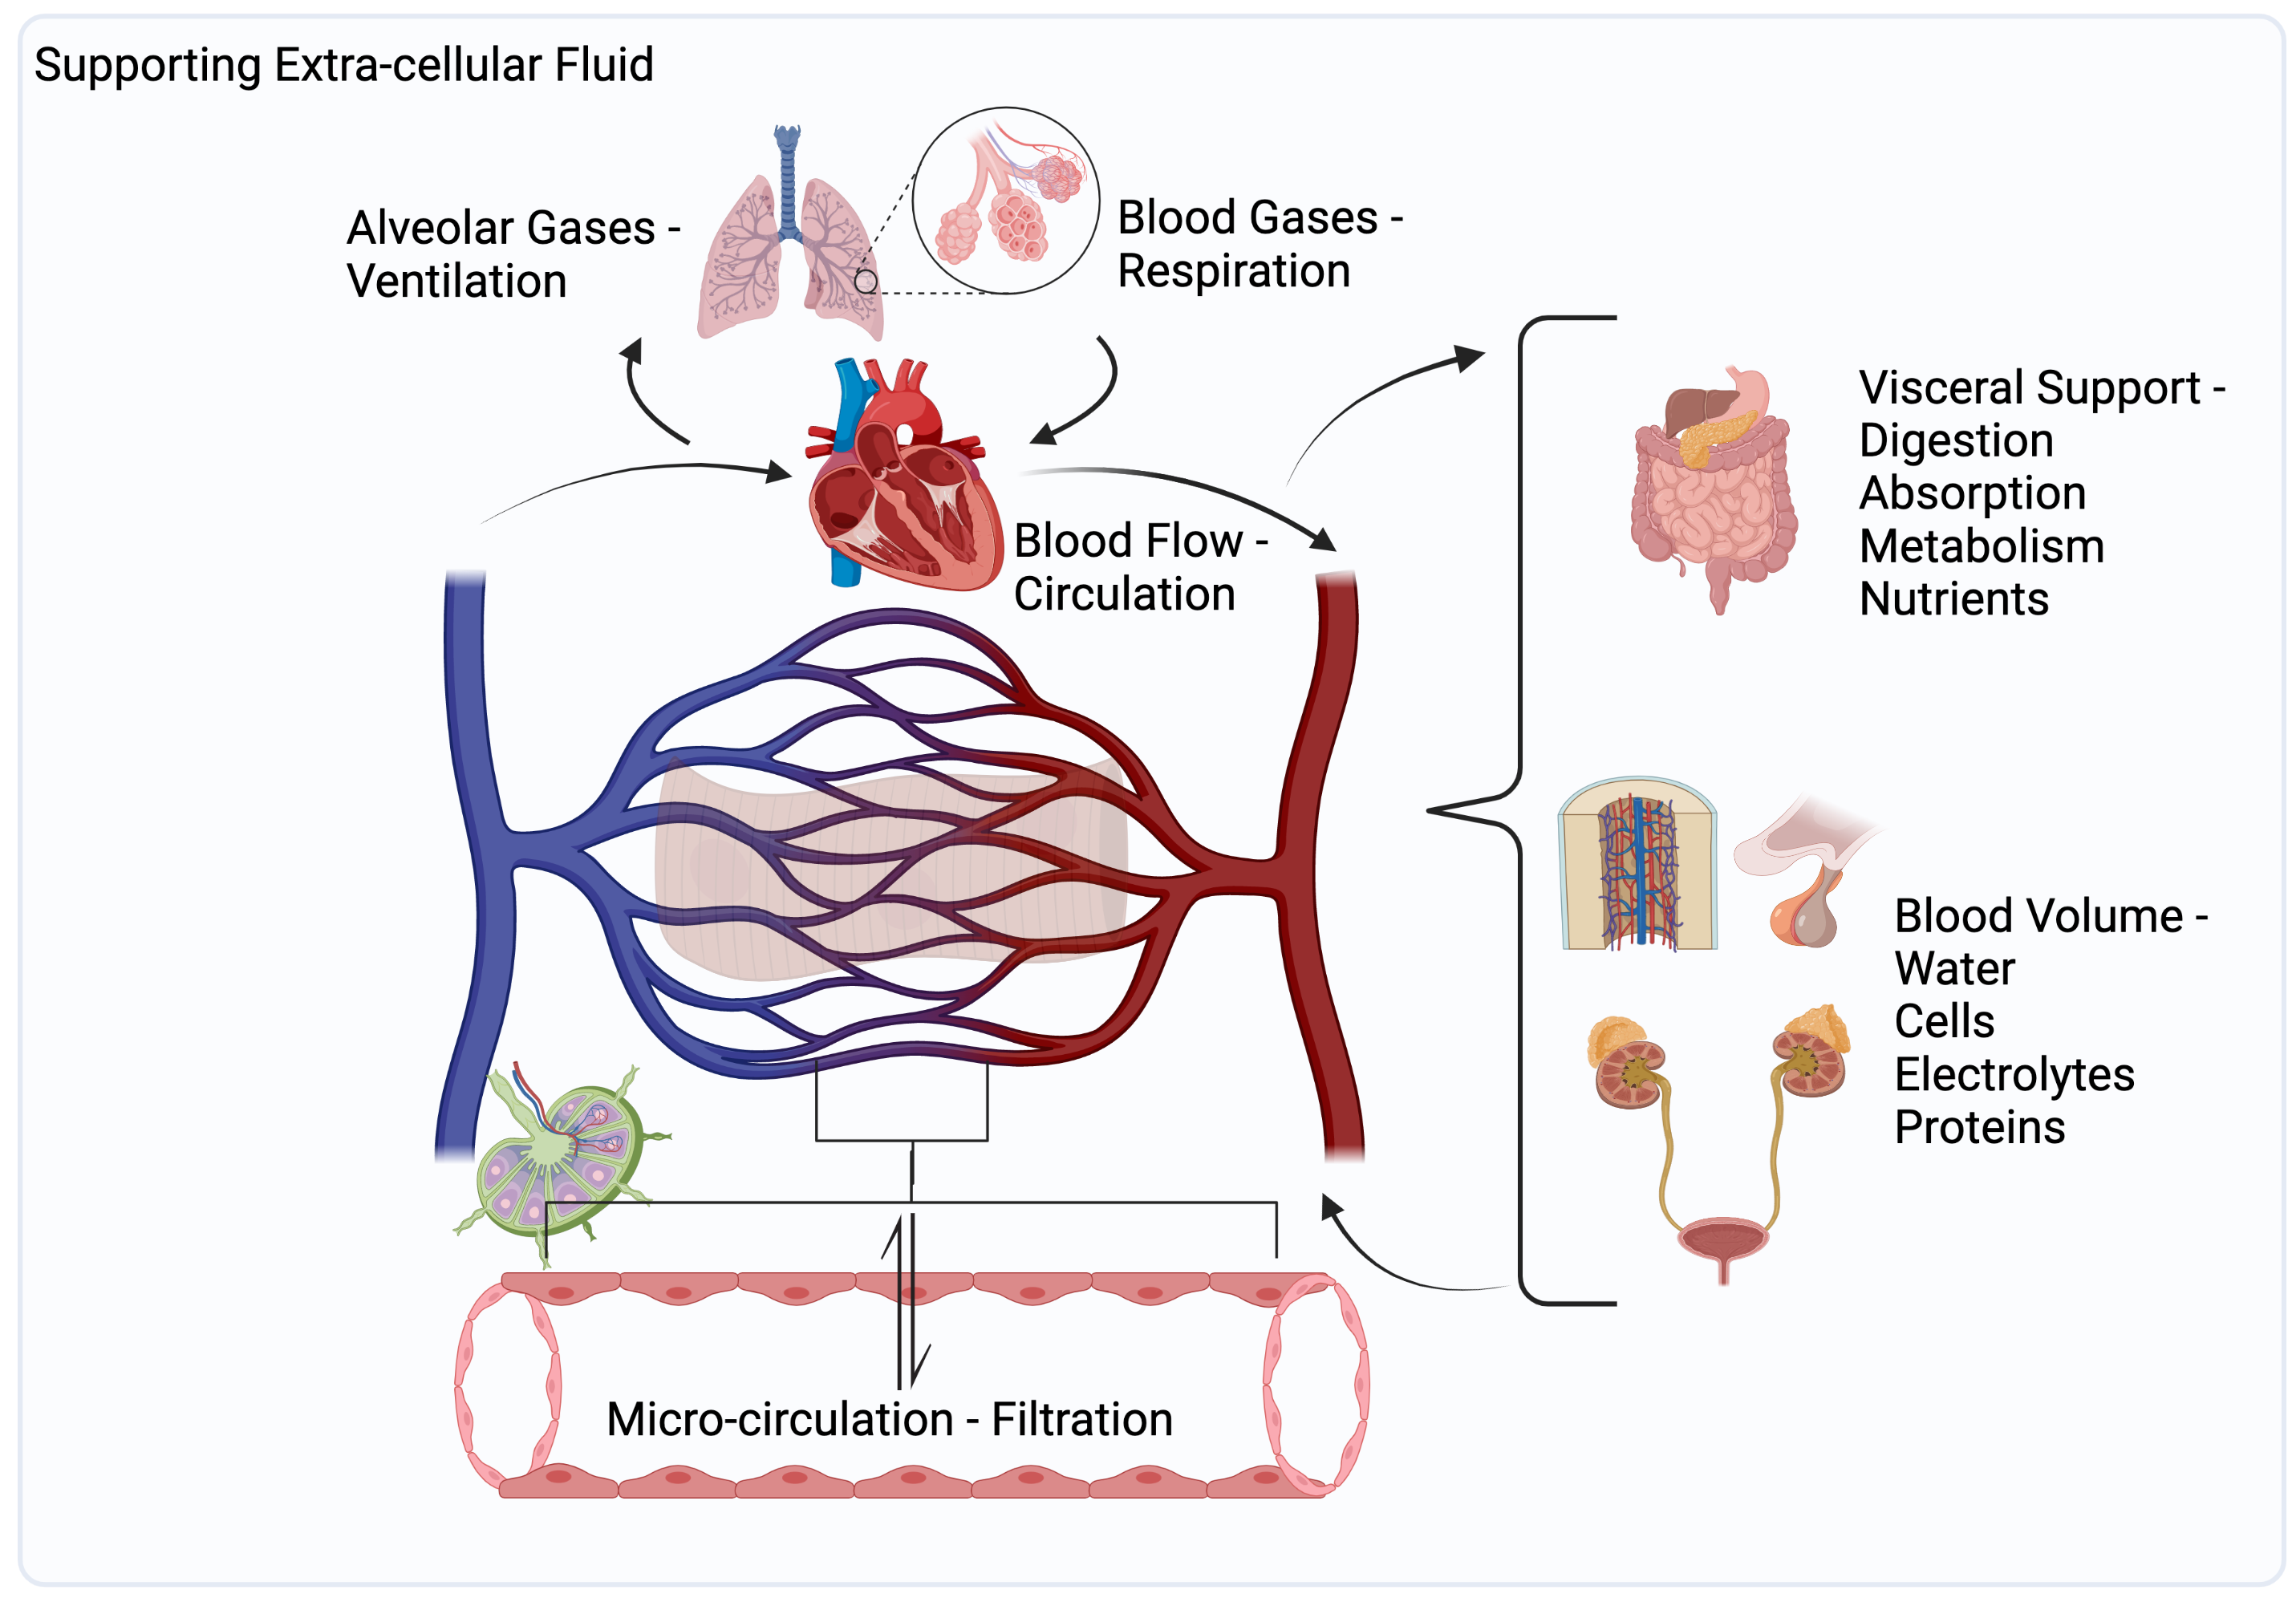
\includegraphics[width=1\linewidth]{./figure/part2_overview.png}
    \caption{Part II: Muscle Support Overview \footnotesize{Created with BioRender.com}}
    \label{fig:part2_overview}
\end{figure}

Together these systems support the ECF and therefore muscle fibers and muscle function. They maintain homeostasis of several important electrolytes (ions, including $H^+$ as measured by pH), nutrients, molecules, water and physical values such temperature. They are integrated with several interactions to provide support across a wide range of muscle demands in a wide range of circumstances, both good and bad.

\section{Extracellular Fluid}

Between 50-70\% of an adult body is fluid. This large variation in the percent of the adult body is based on variations in lean (mostly muscle) tissue. Approximately 2/3 of total body fluid is intracellular (ICF) and 1/3 is extra cellular (ECF). ECF includes two compartments. The vascular compartment includes the circulating blood, and the interstitial (inside tissue) compartment. Exchange of water, ions, nutrients and molecules occurs between the blood and interstitial fluid through the semi permeable capillary membranes in a process called filtration. Exchange between the interstitial fluid and intracellular fluid occurs through the semi permeable cell membrane (muscle fiber cell membrane is the sarcolemma).

Normal values of several important ions, nutrients and molecules are depicted in Figure \ref{fig:ecf}. Vascular and interstitial values are typically equal unless otherwise noted. $O_2$ and $CO_2$ pass easily through both the semipermeable capillary membrane and the semipermeable sarcolemma. Even at rest there is a relatively large gradient for these molecules. 

\begin{figure}[!h]
    \centering
    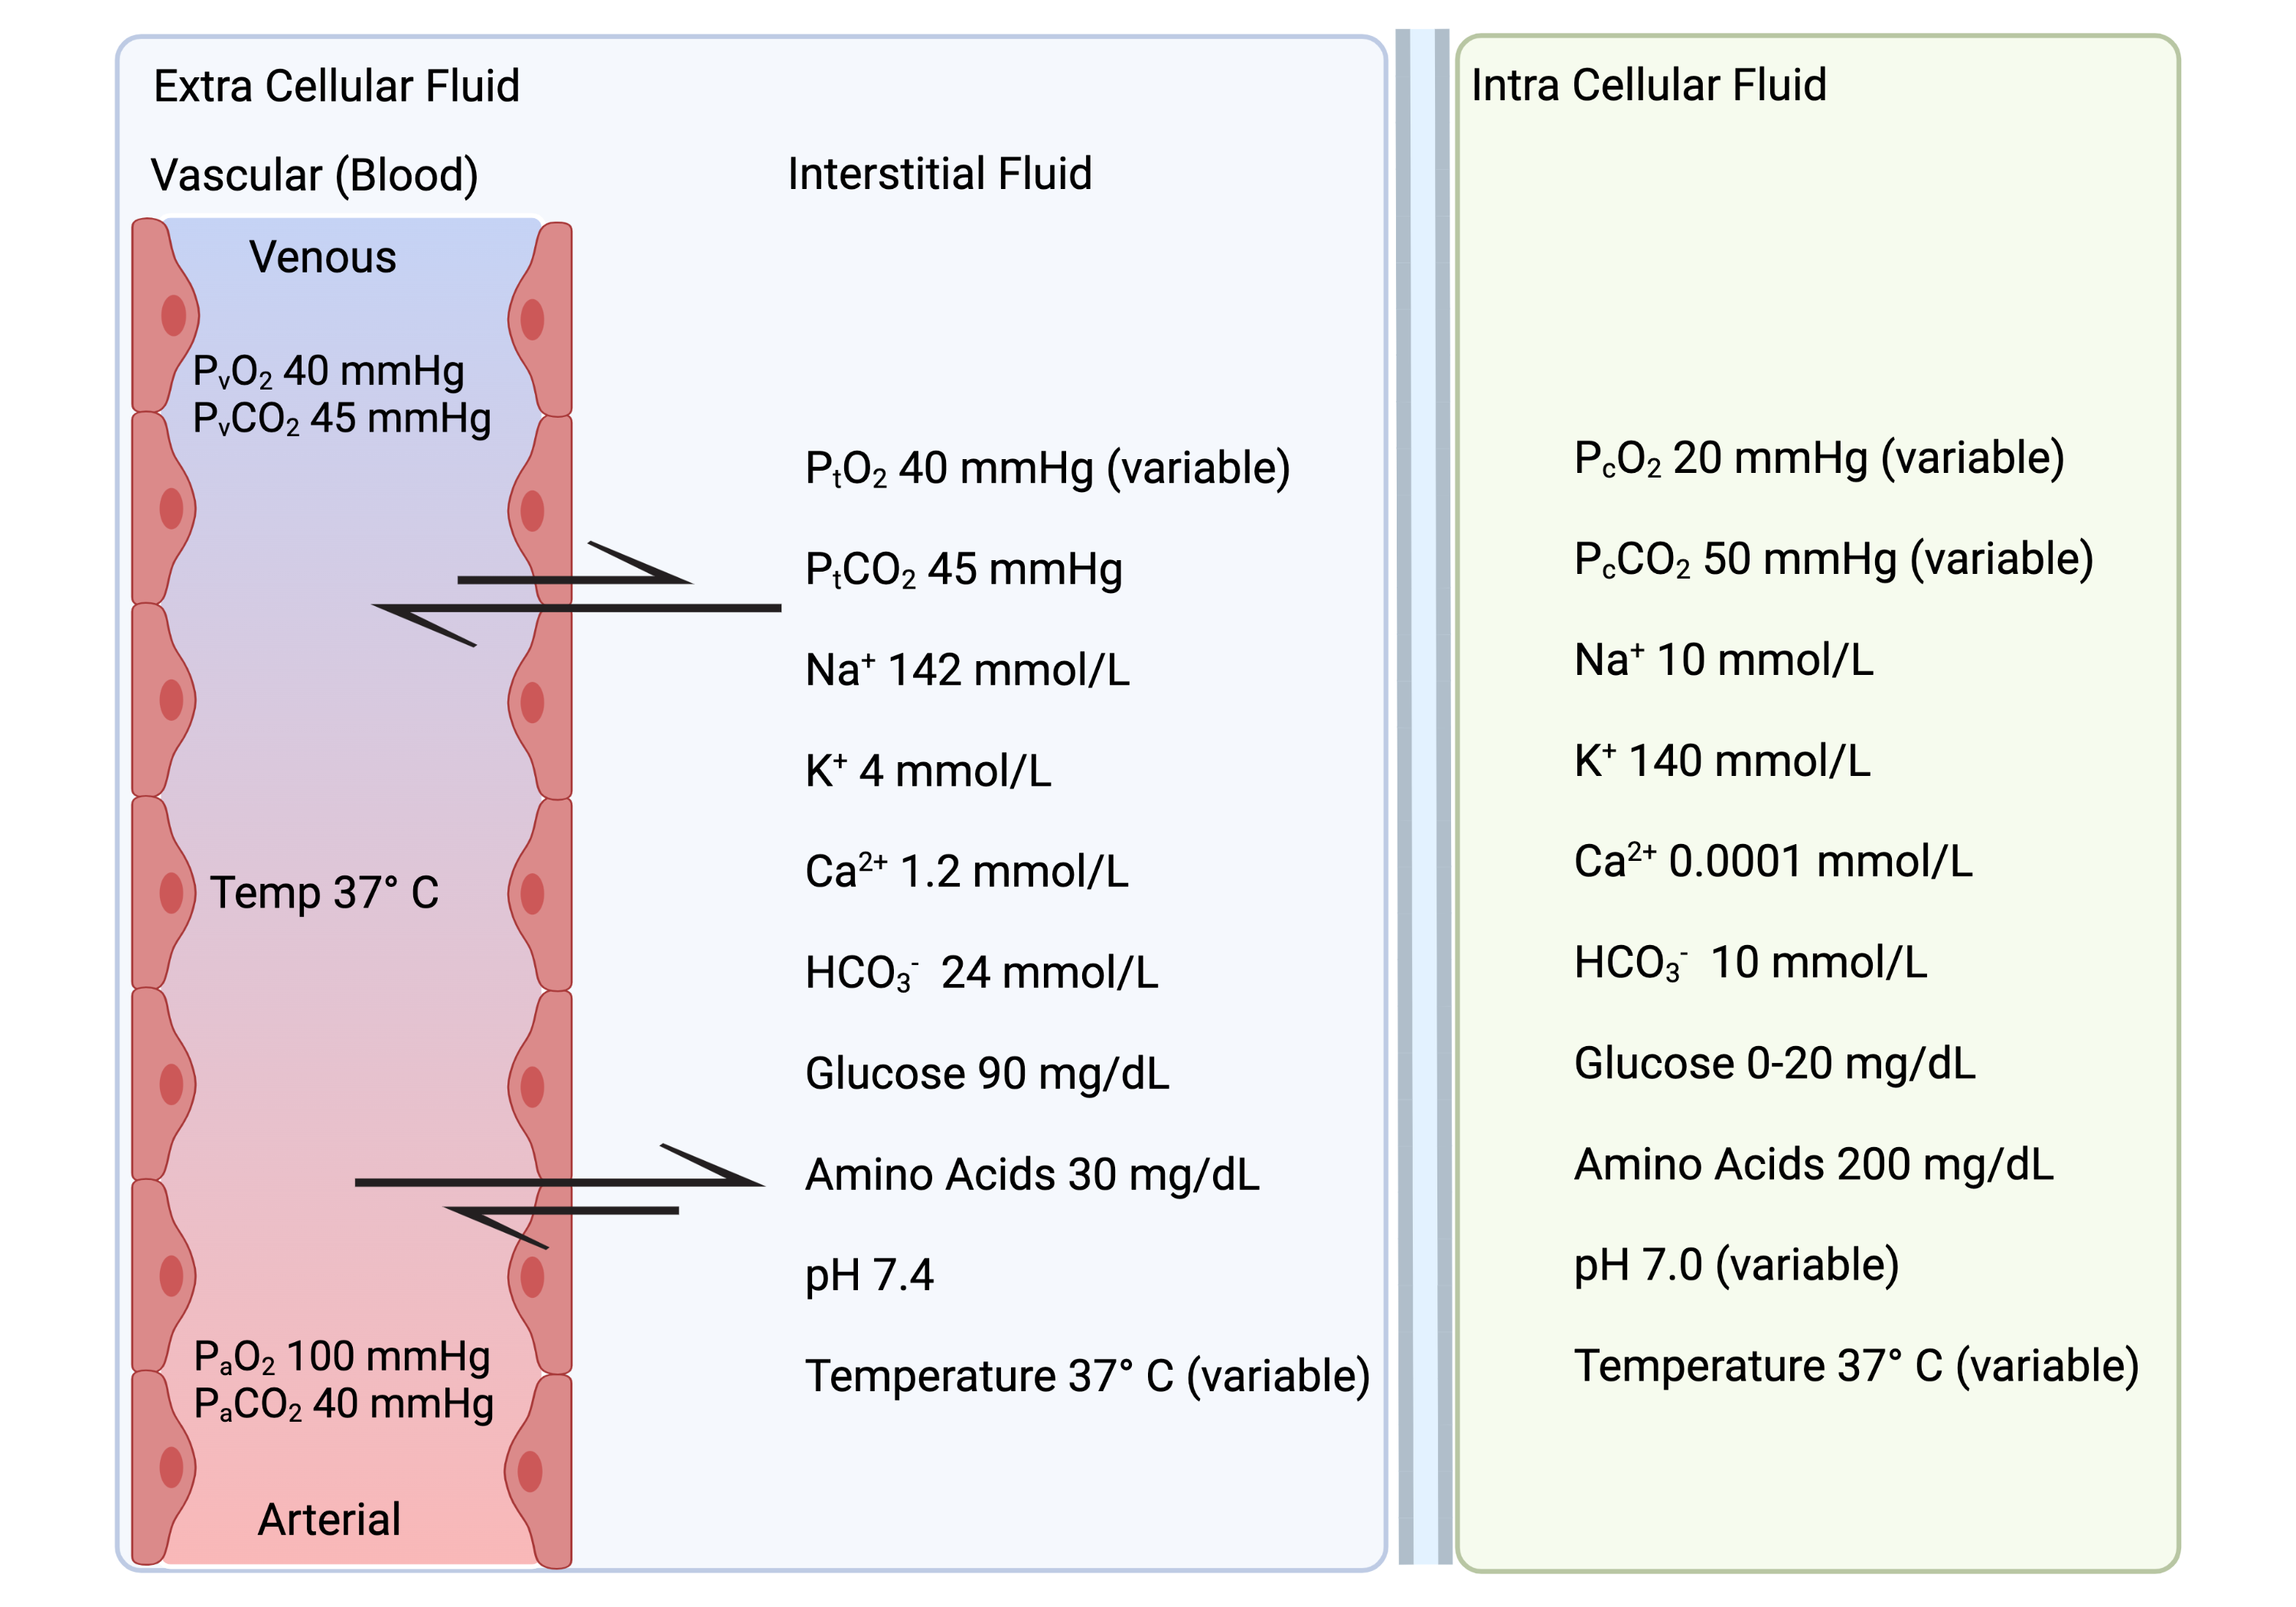
\includegraphics[width=1\linewidth]{./figure/ecf.png}
    \caption{Extra-cellular (Vascular \& Interstitial) and Intra-cellular Fluid \footnotesize{Created with BioRender.com}}
    \label{fig:ecf}
\end{figure}

\begin{table}[h!]
\centering
\begin{tabular}{||c c c c||} 
 \hline
Value & Normal Value & Range & Non-Lethal Limit\\ [0.5ex] 
 \hline\hline
 $P_v O_2$ (mmHg) & 40  & 25-40 & 10-1000 \\
 $P_v CO_2$ (mmHg) & 45 & 41-51 & 5 - 80\\ 
 $Na^+$ (mmol/L) & 142 & 135 - 145 & 115 - 175\\
 $K^+$  (mmol/L) & 4.2 & 3.5 - 5.3 & 1.5 - 9.0\\ 
 $Ca_{2+}$ (mmol/L) & 1.2 & 1.0 - 1.4 & 0.5 - 2.0 \\
 $HCO_3 ^-$ (mmol/L)& 24 & 22 - 29 & 8 - 45 \\
 Glucose (mg/dL)& 90 & 70 - 115 & 20 - 1500 \\
 Acid-Base (pH) & 7.4 & 7.3 - 7.5 & 6.9 - 8.0 \\[1ex] 
 \hline
\end{tabular}
\caption{Normal Range of Values in ECF (\footnotesize{Data from \cite{feher_quantitative_2017}})}
\label{table:ecf_value_ranges}
\end{table}

\paragraph{Micro-circulation of Oxygen \& Carbon Dioxide}

The gradient for $O_2$ from the vascular fluid into the cell because the cell is constantly utilizing $O_2$. The gradient for $CO_2$ from the cell to the vascular fluid since the cell is constantly producing $CO_2$. The other gradient for $O_2$ and $CO_2$ depicted in Figure \ref{fig:ecf} is from the arterial end of the capillary to the venous end of the capillary. As shown, with healthy capillaries, normal capillary blood flow and normal blood the vascular $O_2$ and $CO_2$ partial pressure equilibrate by the time blood reaches the venous end of the capillary. The cellular and interstitial partial pressure for oxygen ($P_c O_2$ \& $P_t O_2$) are variable based on how much $O_2$ is being consumed in the muscle fiber, which is dependent on the rate of ATP regeneration occurring in electron transport (ETC). With a higher than resting ATP regeneration in ETC the $P_c O_2$ will drop, which drops the $P_t O_2$ below 40 mmHg, and then the partial pressure of oxygen at the venous end $P_v O_2$ of the capillary will also drop. $P_v O_2$ will equilibrate to $P_t O_2$. However, the $P_a O_2$ will remain at 100 mmHg as long as the circulation and pulmonary systems are providing the additional support that is required.

Similarly, for ETC to be regenerating ATP at a higher rate, TCA has to be functioning at a higher rate and thus producing more $CO_2$. This results in a higher $P_c CO_2$. However, because $P_t CO_2$ and $P_v CO_2$ equilibrate, as long as the circulation and pulmonary systems are providing the additional support that is required there will not be an increase in either $P_t CO_2$ or $P_v CO_2$.

\paragraph{Temperature}

Temperature is heat unless there is a temperature of 0 degrees Kelvin. Heat is a byproduct of all energetic transformations, including regenerating ATP and hydrolyzing ATP. At rest temperature in muscle fiber equilibrates with that of the body because the flow of heat from the cells into the ECF is moved to the blood and out of the region. Some of the heat also dissipates through the ECF and tissues across the temperature gradient directly out of the body. When core body temperature falls, a reflex action is to shiver, which utilizes muscle activity to generate more heat for sharing with the rest of the body through the transport of ECF. When muscle temperature rises during activity, the circulation of blood carries much of that heat away from the muscle for dissipation throughout the body. As heat rises, more of the circulation is sent to the skin to facilitate this process.

\paragraph{Water}

Cell membranes are permeable to water, but not to the ions. In steady state conditions the osmolarity between the ECF and ICF is approximately equal. Movement of fluid between the ICF and ECF is determined primarily by the osmotic effect. Movement of ions across the cell membrane changes the osmotic balance and results in the movement of water of ECF and ICF electrolytes Of all the ions (electrolytes)

Pressure required to prevent osmosis of water through a semi permeable membrane is osmotic pressure

Osmotic pressure ($\pi$) is directly proportional to the concentration gradient of solutes ($C$), the ideal gas constant ($R$) and absolute temperature ($K = 310^{\circ}$ at body temperature): $\pi = C \cdot R \cdot T$. At body temperature each 1 mOSM/L (milli osmole per liter) difference in solute concentration results in approximately 19.3 mmHg of osmotic pressure. This means 19.3 mmHg of pressure is required to stop the movement of water if there is a 1 mOSM/L concentration gradient, or that 19.3 mmHg of pressure is generated by a difference of 1mOSM/L concentration gradient. Therefore, small differences in solute concentrations across a cell membrane results in rapid osmosis of water.

\begin{figure}[!h]
    \centering
    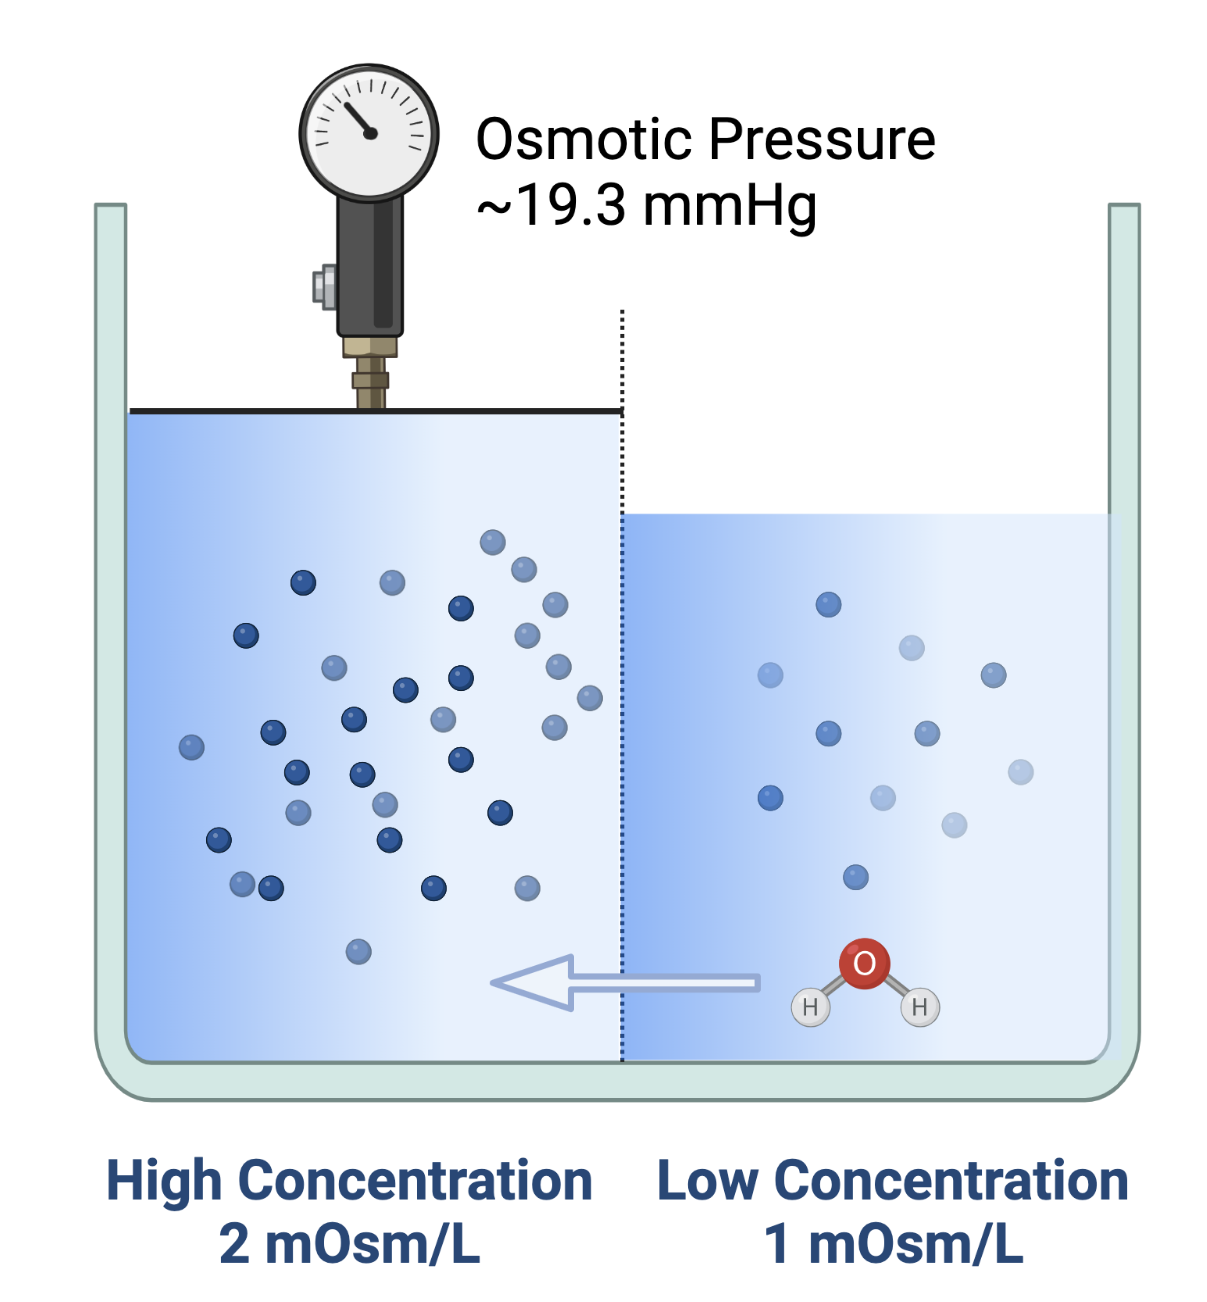
\includegraphics[width=1\linewidth]{./figure/osmotic_pressure.png}
    \caption{Osmotic Pressure \footnotesize{Created with BioRender.com}}
    \label{fig:osmotic_pressure}
\end{figure}

Rapid changes in ICF and ECF can include increases due to large water intake or IV infusions; or decreases (dehydration) associated with sweating, GI fluid loss, excessive urine formation by the kidneys.

Since water moves quickly across the cell membranes the ICF and ECF osmotic pressures quickly equalize. 

Number of osmoles in ECF and ICF remains relatively constant unless solutes are added or lost from the ECF. 

Adding an isotonic solution to ECF- no change in ECF osmolarity, no osmosis, increases ECF volume

Adding hypertonic solution to ECF - ECF osmolarity increases causes osmosis of water out of cells to ECF, increased ECF volume more than already added, decreased ICF volume which increases ICF solute concentration - eventually osmosis of water out of cells stops when osmolarity is equalized

Add hypotonic solution to ECF - ECF osmolarity decreases, causes osmosis of water into cells until osmolarity equalizes both ECF and ICF increase, but ICF to a larger extent



\section{Filtration}
\subsection{Osmosis}

\begin{figure}[!h]
    \centering
    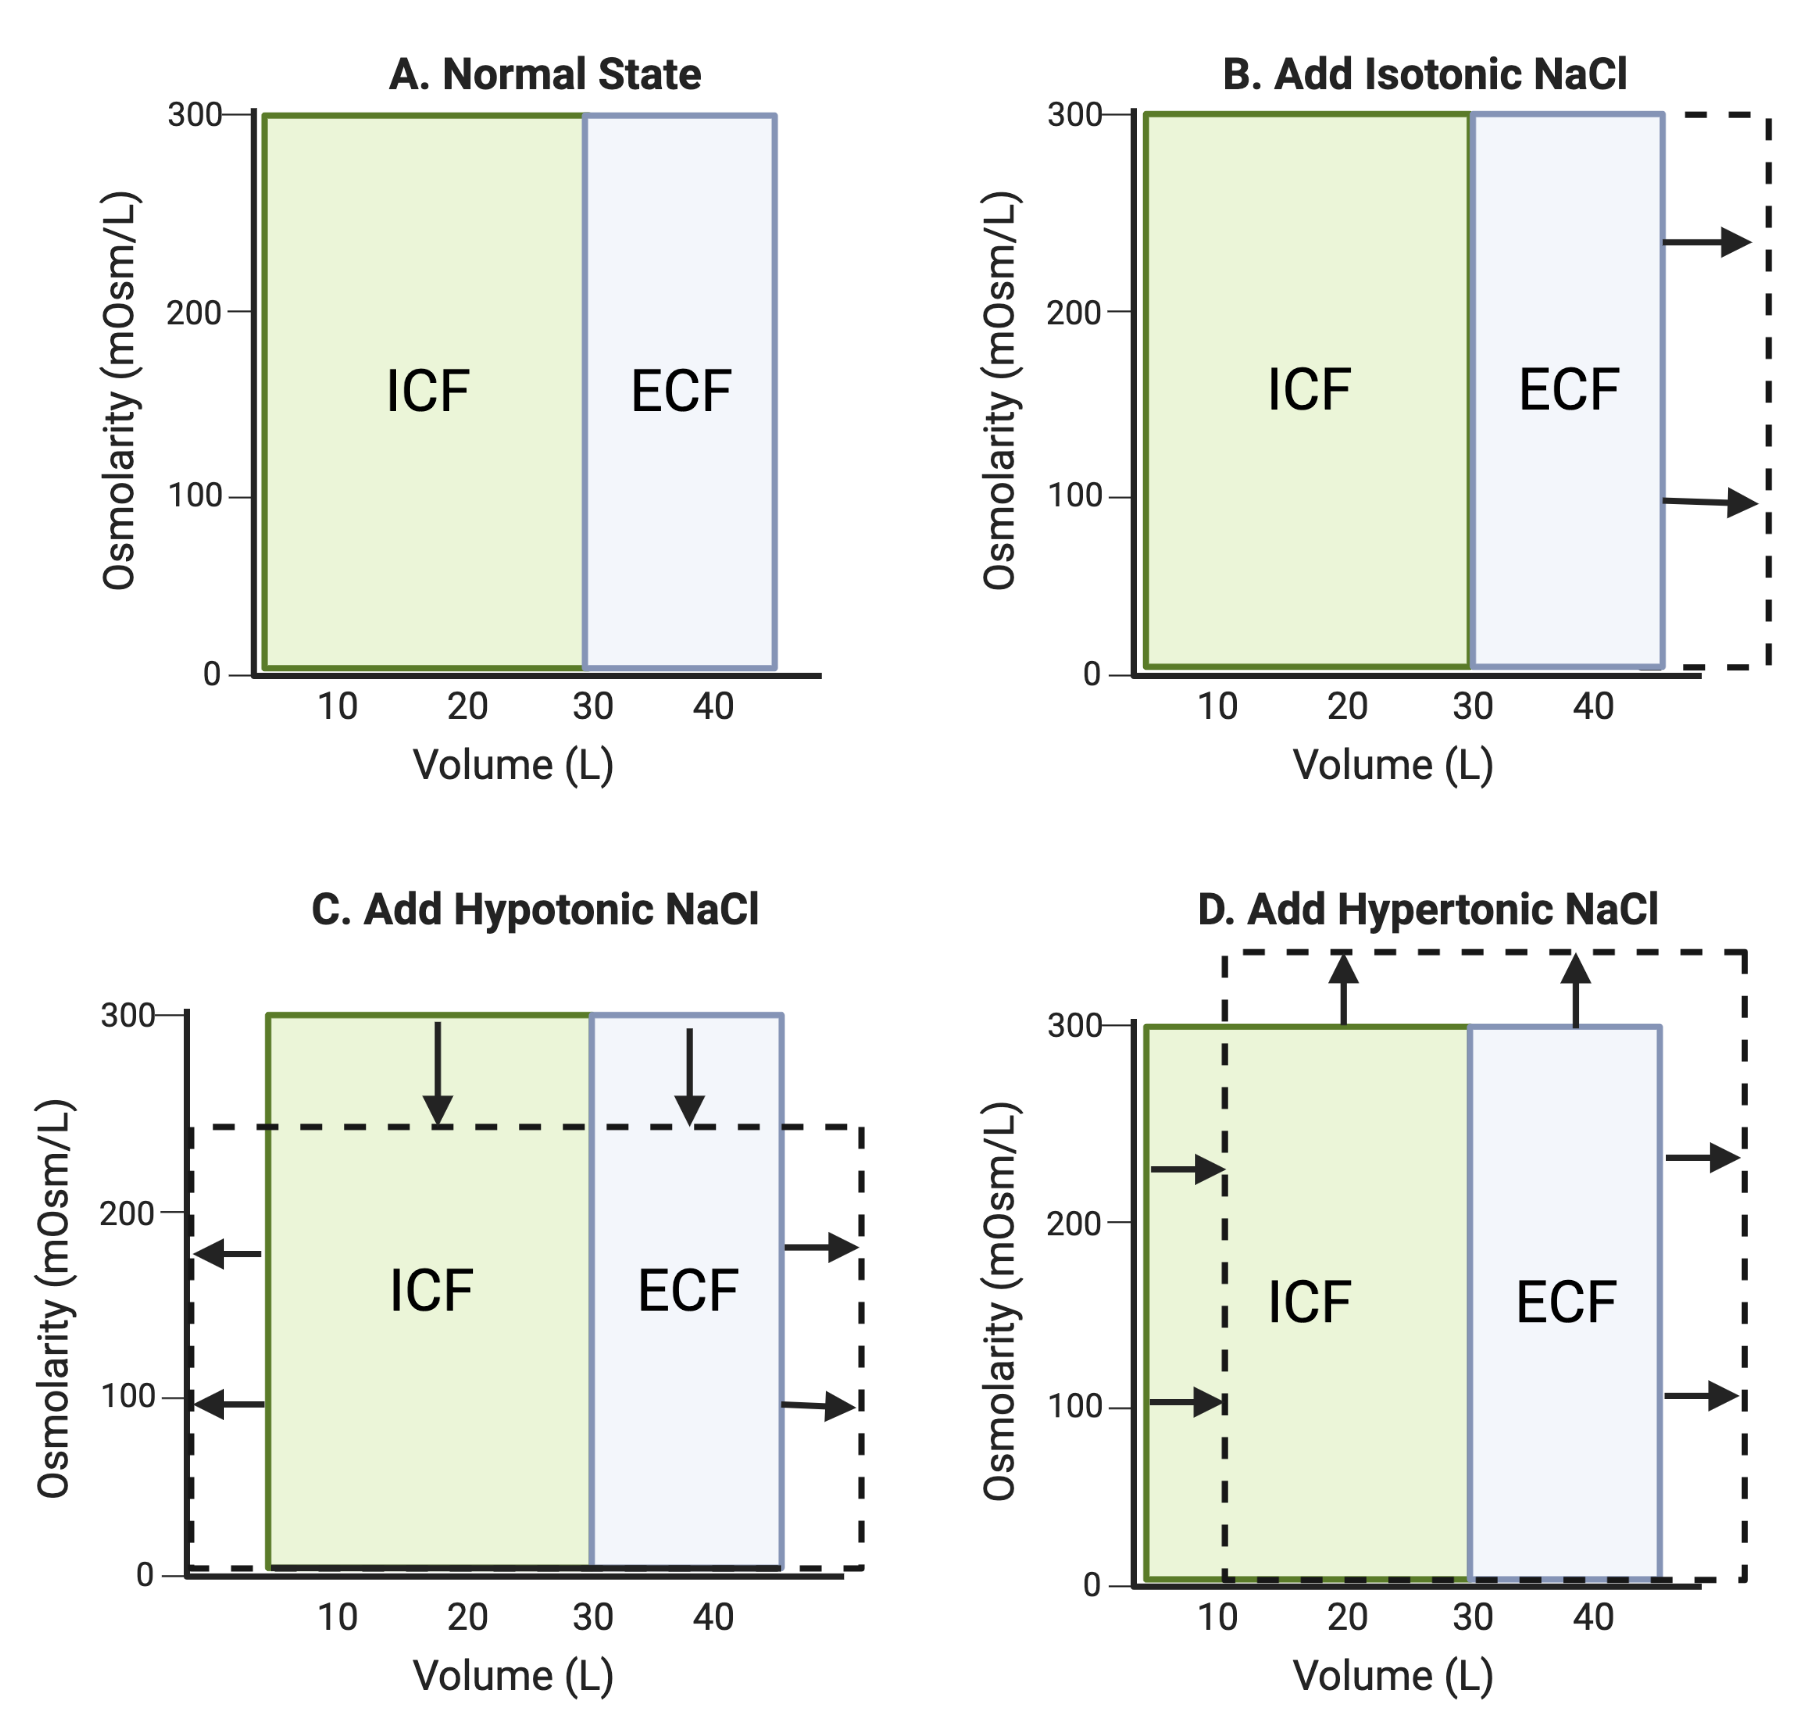
\includegraphics[width=1\linewidth]{./figure/iso_hypo_hypertonic.png}
    \caption{Osmotic Pressure \footnotesize{Created with BioRender.com}}
    \label{fig:iso_hypo_hypertonic}
\end{figure}


\section{Homeostasis}

\subsection{Oxygen \& Carbon Dioxide}

\subsection{Sodium}

\subsection{Potassium}

\subsection{Calcium}

Hypocalcemia, hyperreflexia, muscle cramps, numbness and tingling, twitches
Decreased ECF calcium levels, lowers the threshold potential making it easier to reach threshold for excitation

Hypercalcemia - at high concentrations calcium blocks sodium channels and inhibits depolarization of nerve and muscle fibers, increased calcium raises the threshold for depolarization.[5] This results in diminished deep tendon reflexes (hyporeflexia), and skeletal muscle weakness.

\subsection{Acid Base (pH)}

\subsection{Temperature}

\subsection{Water}



\section{\textit{Clinical Physiology Connections}}

\subsection{Smooth Muscle}

\subsection{Edema}

\subsection{Electrolyte Disturbances}

\subsection{Hyperthermia}

\subsection{Hypotermia}

\printbibliography[heading=subbibintoc]
